\documentclass{article}

% Recommended, but optional, packages for figures and better typesetting:
\usepackage{microtype}
\usepackage{graphicx}
\usepackage{subfigure}
\usepackage{booktabs} % for professional tables

% hyperref makes hyperlinks in the resulting PDF.
% If your build breaks (sometimes temporarily if a hyperlink spans a page)
% please comment out the following usepackage line and replace
% \usepackage{icml2024} with \usepackage[nohyperref]{icml2024} above.
\usepackage{hyperref}


% Attempt to make hyperref and algorithmic work together better:
\newcommand{\theHalgorithm}{\arabic{algorithm}}

% Use the following line for the initial blind version submitted for review:
% \usepackage{icml2024}

% If accepted, instead use the following line for the camera-ready submission:
\usepackage[accepted]{icml2024}

% For theorems and such
\usepackage{amsmath}
\usepackage{amssymb}
\usepackage{mathtools}
\usepackage{amsthm}

% if you use cleveref..
\usepackage[capitalize,noabbrev]{cleveref}

%%%%%%%%%%%%%%%%%%%%%%%%%%%%%%%%
% THEOREMS
%%%%%%%%%%%%%%%%%%%%%%%%%%%%%%%%
\theoremstyle{plain}
\newtheorem{theorem}{Theorem}[section]
\newtheorem{proposition}[theorem]{Proposition}
\newtheorem{lemma}[theorem]{Lemma}
\newtheorem{corollary}[theorem]{Corollary}
\theoremstyle{definition}
\newtheorem{definition}[theorem]{Definition}
\newtheorem{assumption}[theorem]{Assumption}
\theoremstyle{remark}
\newtheorem{remark}[theorem]{Remark}

% Todonotes is useful during development; simply uncomment the next line
%    and comment out the line below the next line to turn off comments
%\usepackage[disable,textsize=tiny]{todonotes}
\usepackage[textsize=tiny]{todonotes}


% The \icmltitle you define below is probably too long as a header.
% Therefore, a short form for the running title is supplied here:
\icmltitlerunning{k-NN on Waveform Dataset}

\begin{document}

\twocolumn[
\icmltitle{Implementing Various k-NN Algorithms and Optimisations using the Waveform Dataset}

% It is OKAY to include author information, even for blind
% submissions: the style file will automatically remove it for you
% unless you've provided the [accepted] option to the icml2024
% package.

% List of affiliations: The first argument should be a (short)
% identifier you will use later to specify author affiliations
% Academic affiliations should list Department, University, City, Region, Country
% Industry affiliations should list Company, City, Region, Country

% You can specify symbols, otherwise they are numbered in order.
% Ideally, you should not use this facility. Affiliations will be numbered
% in order of appearance and this is the preferred way.
\icmlsetsymbol{equal}{*}

\begin{icmlauthorlist}
\icmlauthor{Patrick Barry}{}
\icmlauthor{Buu Dinh Ha}{}
\end{icmlauthorlist}


% You may provide any keywords that you
% find helpful for describing your paper; these are used to populate
% the "keywords" metadata in the PDF but will not be shown in the document
% \icmlkeywords{Machine Learning, ICML}

\vskip 0.3in
]

% this must go after the closing bracket ] following \twocolumn[ ...

% This command actually creates the footnote in the first column
% listing the affiliations and the copyright notice.
% The command takes one argument, which is text to display at the start of the footnote.
% The \icmlEqualContribution command is standard text for equal contribution.
% Remove it (just {}) if you do not need this facility.

%\printAffiliationsAndNotice{}  % leave blank if no need to mention equal contribution
% \printAffiliationsAndNotice{\icmlEqualContribution} % otherwise use the standard text.

\begin{abstract}
    This report will discuss the process of applying various machine learning techniques on the waveform dataset. The techniques and algorithms that will be covered during this report are: k-nearest neighbours (k-NN), data reduction techniques, using the triangle inequality to speed up calculations, and analysing the effect of sampling methods on the dataset.
\end{abstract}

\section{Introduction}
    This report investigates the application of the k-Nearest Neighbors (k-NN) algorithm and several optimization techniques to the waveform dataset. k-NN is a non-parametric learning algorithm widely used for various machine learning tasks.

    This project explores four different methods to improve the performance and efficiency of k-NN: 1) tune the number of neighbours for $k$ using k-fold cross-validation, 2) implement data reduction techniques to improve efficiency, 3) implement the triangle inequality to improve performance, 4) analyse the effects of oversampling and undersampling.

    The waveform dataset contains 5000 examples, 3 classes (equally represented), 20 continuous variables and a optimal Bayesion classification rate of 86\%.


\section{Experimental Set-up}
    \subsection{Data Exploration}
        To get a better understanding of the dataset, we first explored the data to identify potential features for removal and any outlying examples that might skew our results.

        All input features are represented as floating-point numbers. The target variable, located in column 21, has the integer values: \{0, 1, 2\}.

        Initially, the dataset was split into training and test sets, with an 80/20 split. We then separated the input features (represented as $X$) and the target variable (represented as $y$) for both the training and test sets.


        Figure \ref{fig:corr_matrix} shows the correlation matrix for the features in the training set, including both $X$ and $y$. The visualisation shows some distinct areas of higher positive and negative correlations, especially surrounding the diagonal. Several features have a positive or negative correlation of more than 0.7, which suggests that dimensionality reduction techniques, such as Principal Component Analysis (PCA), could be effectively applied.

        \begin{figure}[h]
            \centering
            \begin{minipage}[t]{0.7\linewidth}
                \centering
                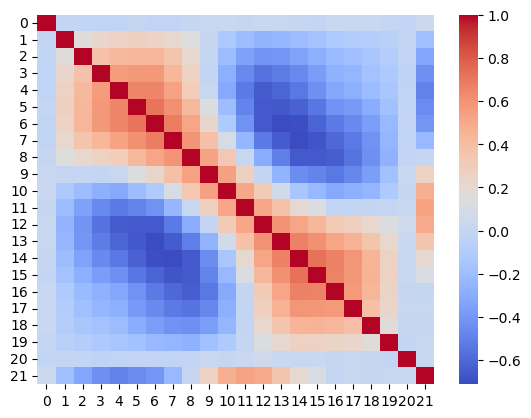
\includegraphics[width=\linewidth]{figures/correlation_matrix.png}
                \caption{Correlation Matrix for Features in Waveform Training Set}
                \label{fig:corr_matrix}
            \end{minipage}%
        \end{figure}

    \subsection{Data Manipulation}
        \label{sec:data_manip}
        To allow comparative analysis between features and simplify Euclidean distance calculations for kNN, we standardised the data using the z-score. It is important to standardise the test data using the mean and standard deviation from the training data. This prevents data leakage, which is when test set data influences the training set, leading to unreliable estimates of generalised error.

        Using the standardised data, we can use box-plots to visually search for outliers. Illustrated in Figure \ref{fig:box_features}, a box-plot shows the interquartile range (IQR) within the box, where 50\% of the data lies. The whiskers, extending from the box, show the values within 1.5 times the IQR for both lower and upper quartiles. Therefore the values outside the whiskers are the potential outliers. In the waveform dataset, features 5 to 16 have fewer outliers, indicating more stability, while the other features have higher variability in their data, with more outliers above and below the mean. It is likely that these features with more variation have a larger impact in differentiating the examples.

        It is difficult to determine if there are significant outliers in the data from this plot alone. An example may have an outlier value for one feature but lie in the typical range for all other features.

        \begin{figure}[h]
            \centering
            \begin{minipage}[t]{0.7\linewidth}
                \centering
                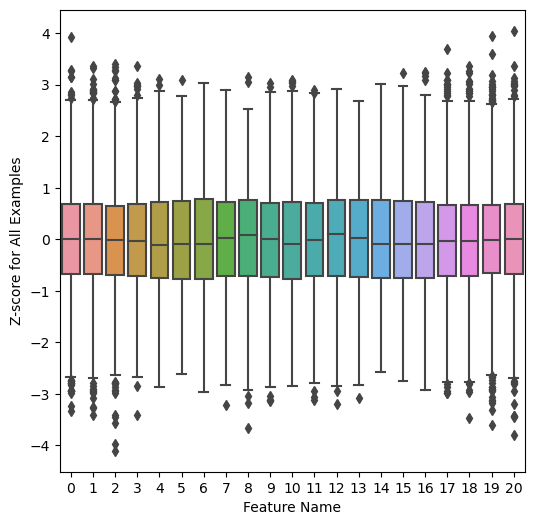
\includegraphics[width=\linewidth]{figures/box_plot_features.png}
                \caption{Correlation Matrix for Features in Waveform Training Set}
                \label{fig:box_features}
            \end{minipage}%
        \end{figure}


\subsection{Tuning k of k-NN by Cross Validation}
\label{sec:cross_val}
To prevent the recomputation of distance when performing k-NN, first we computed the Euclidean distance matrix for each pair of points in the training set with the function \texttt{ComputeDistanceMatrix}, where each entry $D[i,j]$ is the distance between point $i$ and $j$.


We performed 10 folds cross validation. \texttt{KFoldIndices} function takes an input train set and splits it into 10 folds. This function creates 10 folds, each fold containing one training set and one validation set, which are both created from the training set.

Given folds $\mathcal{F}$, we looped through each fold. First, we computed the distance sub-matrix between the validation set and all datasets $\mathcal{D}_{\text{val}}$. An empty prediction array $\mathcal{P}$ was initialized. For each $x$ in $\mathcal{X}_{\text{val}}$, we used \texttt{GetNeighbors} to find the k-NN, storing indices in $\mathcal{N}$. \texttt{KnnPrediction} used $\mathcal{N}$ and $\mathcal{Y}_{\text{train}}$ to retrieve neighbor labels and perform majority voting, yielding prediction $y_{\text{pred}}$, which was added to $\mathcal{P}$. Actual labels $\mathcal{Y}_{\text{val}}$ were obtained using $\mathcal{Y}_{\text{train}}$ and $\mathcal{X}_{\text{val}}$. \texttt{AccuracyMetric} compared $\mathcal{Y}_{\text{val}}$ and $\mathcal{P}$, incrementing a counter for each matching prediction. Accuracy was calculated as $accuracy = \frac{N_{\text{correct}}}{N_{\text{total}}} \times 100$ and added to $\mathcal{A}$. After k-folds Cross Validation, we obtained a list of accuracies $\mathcal{A}$.

Pseudo-code for the implementation is Algorithm \ref{alg:k_folds_cross_validation}.

Next, we tuned $k$ (number of neighbors) to find the optimal value, which maximizes the accuracy of the model. Since we trained on the train data, $k =\sqrt{n} = \sqrt{4000} \approx 63$ is a good starting point. Thus, we looped over $k$ from 1 to 100. For each $k$, we ran 10-folds Cross Validation to get the list of accuracies for 10 folds $\mathcal{A}$ and computed the mean accuracy. We tracked the best $k$ that gives the highest accuracy, which is the optimal value that we are looking for.

\subsection{Data Reduction Implementation}
\label{sec:data_reduction}
    To increase the performance of the k-NN algorithm, especially in terms of computation time, it is necessary to perform data reduction on the dataset. The data reduction technique we implemented is executed in two steps as presented in Hart 1968 \cite{hart1968condensed}. The first step removes the outliers from the data, outlined in the algorithm \ref{alg:remove_outliers}. This algorithm uses the 1-NN classifier for outlier detection based on the fact that outliers are often misclassified by their single nearest neighbor.


    The second step removes all points that are not necessary to classify new examples, outlined in the algorithm \ref{alg:remove_redundancy}. This algorithm starts with an empty set, $STORAGE$, and iteratively adds misclassified points to it. In doing this, it keeps only the points that are required to define the decision boundaries between classes.



\subsection{Speeding up the calculation}

Given a test point, brute force 1-NN computes the distance from the test point to every point in the train set and selects the closest point as its nearest neighbor. We implemented a function that takes an input 3 datasets $\mathcal{X}_{\text{train}}$, $\mathcal{Y}_{\text{train}}$, $\mathcal{X}_{\text{test}}$ and returns the list of predicted labels $\mathcal{P}$ for the test set. For each test point in $\mathcal{X}_{\text{test}}$, we calculate the distance to all training points in $\mathcal{X}_{\text{train}}$ and choose the minimum. The label associated with this minimum value in $\mathcal{Y}_{\text{train}}$ is stored in $\mathcal{P}$. The pseudocode of Brute Force 1-NN is Algorithm \ref{alg:brute_force_1nn}.

The Triangle Inequality 1-NN algorithm aims to increase the performance of Brute Force by using the triangle inequality to eliminate points that cannot be the nearest neighbor. We implemented a function that takes the same 3 input datasets as Brute Force and returns predictions $\mathcal{P}$ also. The pseudocode can be found in Algorithm \ref{alg:triangle_inequality_1nn}. For each test instance, we set the mininum distance equal to distance to the first training instance. We then iterate through the remaining training examples. If the distance from the test example to the training is larger than the minimum distance, we will perform the triangle inequality. We calculate two spheres, bounds are defined by a lower bound and lower bound. Then we filtered candidates using the Triangle Inequality. To do this, first we computed the distance between the current candidate and the remaining candidate using the distance matrix $\mathcal{D}$. Then, we just kept the candidates that its distances to the remaining candidate is larger than the lower bound of the sphere and smaller than the upper bound of the sphere.

For each test instance $x_{\text{test}}$ in the test set $X_{\text{test}}$, we initialized the minimum distance $d_{\text{min}}$, the label of the nearest neighbor and the indices of all candidate neighbors $\mathcal{C}$ (initially containing all training points). We did a loop through every candidate index, selected the first candidate $i$ from $\mathcal{C}$. Then, we computed the Euclidean distance $d_{\text{candidate}}$ between the current test instance $x_{\text{test}}$ and the $i$-th train instance $x_{\text{train}}[i]$. The sphere bounds are defined by a lower bound and lower bound. Then we filtered candidates using the Triangle Inequality. To do this, first we computed the distance between the current candidate and the remaining candidate using the distance matrix $\mathcal{D}$. Then, we just kept the candidates that its distances to the remaining candidate is larger than the lower bound of the sphere and smaller than the upper bound of the sphere. And if $d_{\text{candidate}}$ is smaller than $d_{\text{min}}$, we will update the value of $d_{\text{min}}$ and set the label of the nearest neighbor to the label of $x_{\text{train}}[i]$. After all candidates are processed, we appended the label of the nearest neighbor to $\mathcal{P}$. Finally, after processing all test points, we returned the list $\mathcal{P}$. The pseudocode of Triangle Inequality 1-NN is Algorithm \ref{alg:triangle_inequality_1nn}.




\subsection{Sampling Methods}
    \label{sec:sampling_methods}
    Sampling is commonly used in imbalanced datasets to ensure all classes have an equal representation of examples \cite{mohammed2020}. The waveform dataset is already balanced, with each class representing approximately one-third of the data, so we are implementing sampling methods to artificially create imbalance and investigate the effects on k-NN's performance. We will evaluate using the best $k$ found in Section \ref{sec:cross_val}.

    We implemented two sampling methods: undersampling and oversampling. Undersampling a dataset takes the majority class and randomly removes examples until the dataset is balanced. We tested k-NN using a training and validation set with various levels of imbalanced datasets. We also compared the effect of undersampling each class separately.

    Oversampling involves randomly duplicating examples from the minority class. Each example in the minority class can be duplicated more than once, leading to a high risk of overfitting. We performed the same tests on the oversampled datasets as on the undersampled ones.

    Another sampling method that will not be covered in this report is called SMOTE. This is based on oversampling and aims to reduce the risk of overfitting by generating artifical data points.

    The results of these experiments are presented in Section \ref{sec:sampling_results}, where we compare the performance of k-NN across the various undersampled and oversampled datasets using metrics such as accuracy and F1-score.


\section{Result Analysis}
\subsection{Tuning k of k-NN by Cross Validation}

We plot the accuracy of the implemented k-NN classifier in figure \ref{fig:knn_cross_validation}. The accuracy steadily increases as k rises from $k = 1$ to larger values, reaching a peak when $k = 86$, achieving 85.67\%. This result suggests that the implementation performed as expected, since it is very close to the theoretical Bayes optimal rate (86\%). For small $k$ ($k < 10$), the accuracy fluctuates drastically, which shows that the classifier has high variance at this point, a sign of overfitting. This result can be expected since for small $k$, the classifier closely follows the train data, leading to poor generalization. The curve becomes stable and slightly fluctuates after $k = 30$. This implies that the model's variance is decreasing, and it is reaching the limit because the noise in the dataset prevents it from reaching the optimal Bayes rate.

\begin{figure}[h]
    \centering
    \begin{minipage}[t]{0.8\linewidth}
        \centering
        \includegraphics[width=\linewidth]{figures/knn_cross_validation.png}
        \caption{Accuracy vs Number of neighbors ($k$) for k-NN}
        \label{fig:knn_cross_validation}
    \end{minipage}%
\end{figure}

\subsection{Data Reduction}
    Here, the data reduction algorithms outlined in \ref{sec:data_reduction} are implemented. The first step, removing outliers, reduced the dataset size from 4000 to 3176, identifying 824 outliers, which represents approximately 20\% of the original data. This aligns with the box-plots from Section \ref{sec:data_manip} which showed many features had a large amount of outliers.

    The second step of the algorithm further reduced the dataset by 671 examples, making the final reduced size 2511. The data reduction algorithm has therefore removed approximately 37\% of the training set. To evaluate the impact of this reduction on the performance of the k-NN classifier, we compared the accuracy of 1-NN and k-NN using the best k from Section \ref{sec:cross_val} on the test set, using both the original and reduced training set.

    Table \ref{reduction-table} shows the results of this comparison. There has been no significant loss of information that leads to a decrease in accuracy. The slight improvement in the accuracy of 1-NN on the reduced dataset could be explained by the lack of outliers in the reduced dataset, which 1-NN can be particularly affected by. Meanwhile the slight decrease in accuracy for k-NN could be due to the best k being tuned for the original dataset. It is possible that tuning a new k for the reduced dataset would improve the test accuracy.

    \begin{table}[t]
    \label{reduction-table}
    \vskip 0.15in
    \begin{center}
    \begin{small}
    \begin{sc}
    \begin{tabular}{lcccr}
    \toprule
    Data set & 1-NN & k-NN \\
    \midrule
    Original Training Set  & 75.1\% & 84.3\%  \\
    Reduced Training Set   & 75.7\% & 83.7\%  \\
    \bottomrule
    \end{tabular}
    \end{sc}
    \end{small}
    \end{center}
    \caption{Classification accuracies for 1-NN and k-NN before and after data reduction.}
    \vskip -0.1in
    \end{table}

\subsection{Speeding Up the Calculation}

After performing Brute Force 1-NN and Triangle Inequality 1-NN, we got the computation time for Brute Force around 0.1 seconds and for Triangle Inequality it is around 7 seconds, which is much higher than Brute Force. The computation time for each iteration is shown in figure \ref{fig:brute_force_triangle_inequality}, which supports this result. This is because, at each step, Triangle Inequality filters the list of candidate points by checking if they lie within the sphere bounds or not. This requires logical operations and array indexing on the set of candidate points, which takes more time than a simple computation of distances, as in Brute Force. Another reason is that, when we printed out the filtered candidates (those lie inside the upper bound and lower bound), actually Triangle Inequality does not filter too many candidates. Thus, the algorithm reverts to Brute Force performance but with additional computation.

\begin{figure}[h]
    \centering
    \begin{minipage}[t]{0.8\linewidth}
        \centering
        \includegraphics[width=\linewidth]{figures/brute_force_triangle_inequality.png}
        \caption{Computation time for each test point (iteration)}
        \label{fig:brute_force_triangle_inequality}
    \end{minipage}%
\end{figure}

\subsection{Sampling Methods}
    \label{sec:sampling_results}
    \subsubsection{Sampling with best $k$}
        We implemented the sampling methods outlined in Section \ref{sec:sampling_methods} to investigate their impact on k-NN classifier performance. The dataset was initially split into a training set (3000 examples), a validation set (1000 examples), and a test set (1000 examples). Before applying k-NN, we standardized the test set using the mean and standard deviation calculated from the training set.

        To test undersampling, we tested the accuracy on varying percentages of removal, from 0\% (no removal) up to 100\% (complete removal of the class). The results are shown in Figure \ref{fig:undersample}. The removal of class 2 from the dataset has the biggest impact on the test accuracy, which could suggest that there is a slightly higher representation of class 2 in the test set. Meanwhile removing class 1 had the least effect on the k-NN accuracy, suggesting that it may have a lower representation in the test set.

        \begin{figure}[h]
            \centering
            \begin{minipage}[t]{0.8\linewidth}
                \centering
                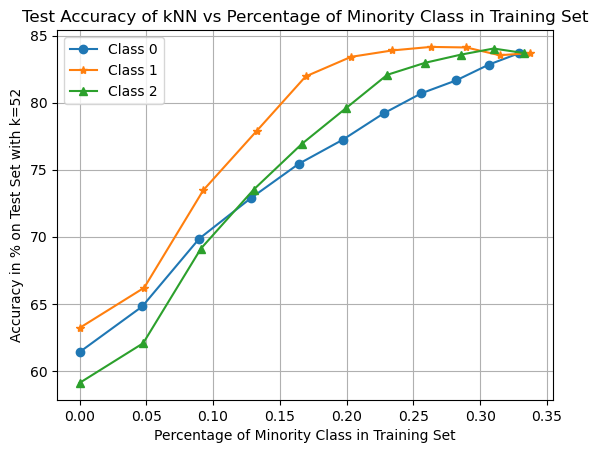
\includegraphics[width=\linewidth]{figures/undersample.png}
                \caption{Accuracy on Test Set vs Percentage of Class in Training Set}
                \label{fig:undersample}
            \end{minipage}%
        \end{figure}

        We then tested the effects of oversampling on classifier accuracy. We increased the number of examples in each class by varying percentages, from 0\% (no oversampling) up to 100\% (twice as many examples of class). The percentage corresponds to the increase in the number of examples relative to the original count of that class in the training set. The results are shown in Figure \ref{fig:oversample}. These results corroborate with those of undersampling, with the oversampling of class 1 leading to a decrease in accuracy. Notably, oversampling both class 0 and class 2 temporarily increases the accuracy on the test set. This could suggest that both class 0 and class 2 are have a higher representation in the test set than class 1.

        To further investigate the class distribution in the test set, we visualized the representation of each class, as shown in Figure \ref{fig:test_dist}.

        \begin{figure}[h]
            \centering
            \begin{minipage}[t]{0.8\linewidth}
                \centering
                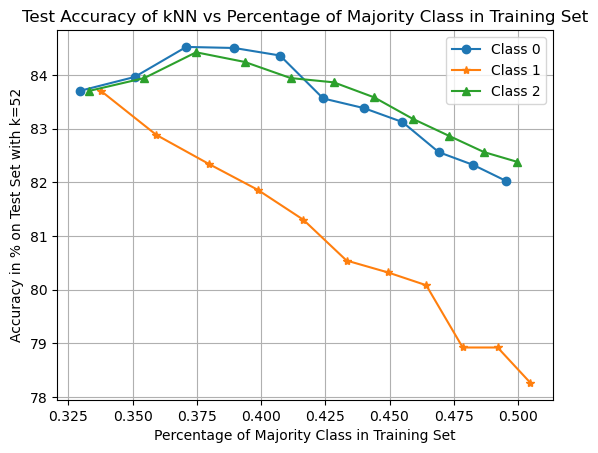
\includegraphics[width=\linewidth]{figures/oversample.png}
                \caption{Accuracy on Test Set vs Percentage of Class in Training Set}
                \label{fig:oversample}
            \end{minipage}%
        \end{figure}

        The test set distribution confirms our hypothesis that class 2 has the lowest representation. It also reveals that class 0 and and class 1 have roughly an equal number of examples in the test set, which is consistent with the oversampling plot.

        \begin{figure}[h]
            \centering
            \begin{minipage}[t]{0.8\linewidth}
                \centering
                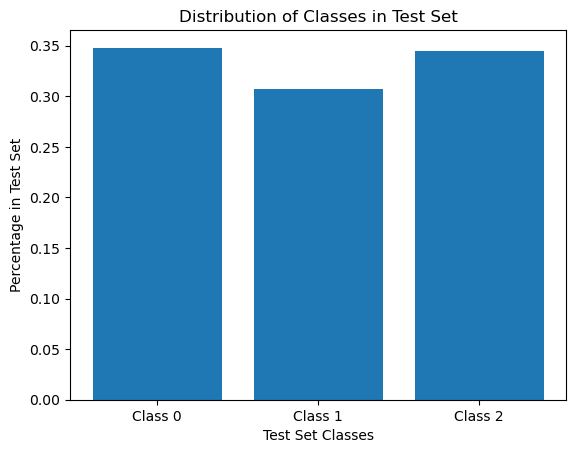
\includegraphics[width=\linewidth]{figures/distribution_test.png}
                \caption{Representation of each class in the test set}
                \label{fig:test_dist}
            \end{minipage}%
        \end{figure}

        Ideally, the test set distribution should mirror the class distribution of the original dataset. A method to implement this is called stratified sampling, which ensures all splits maintain the same distribution. However, this has not been implemented in the project.

    \subsubsection{Sampling using F-Measure to Tune $k$}
        In this section, we use the F-measure to tune the best $k$ for each sampling rate. First, we must apply each sampling rate from 0\% to 100\% in increments of 10\% to each class individually, creating a range of different datasets. Next, we can tune $k$ by testing a range of $k$ values from 1 to 60 against the F-measure on the validation set. The $k$ value with the highest F-measure is selected as the best performer.

        Figure \ref{fig:f_under} shows the results of this process for undersampling. Unexpectedly, using the F-measure to tune $k$ does not improve the accuracy of the classifier on the test set. The highest test accuracy achieved is approximately 81\%, and the lowest is worse than the results obtained in the initial undersampling (Figure \ref{fig:undersample}).

        \begin{figure}[h]
            \centering
            \begin{minipage}[t]{0.8\linewidth}
                \centering
                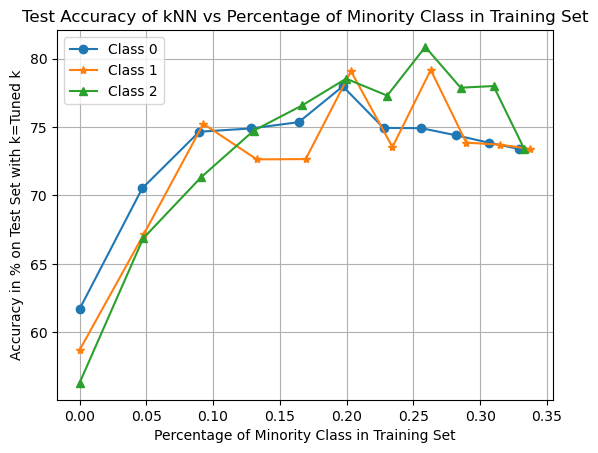
\includegraphics[width=\linewidth]{figures/f_measure_under.png}
                \caption{Representation of each class in the test set}
                \label{fig:f_under}
            \end{minipage}%
        \end{figure}

        Figure \ref{fig:f_over} shows the graph for the oversampling method. The results are consistent with the undersampling graph: using the F-measure to tune $k$ does not improve the classification accuracy on the test set and generally decreases it.

        \begin{figure}[h]
            \centering
            \begin{minipage}[t]{0.8\linewidth}
                \centering
                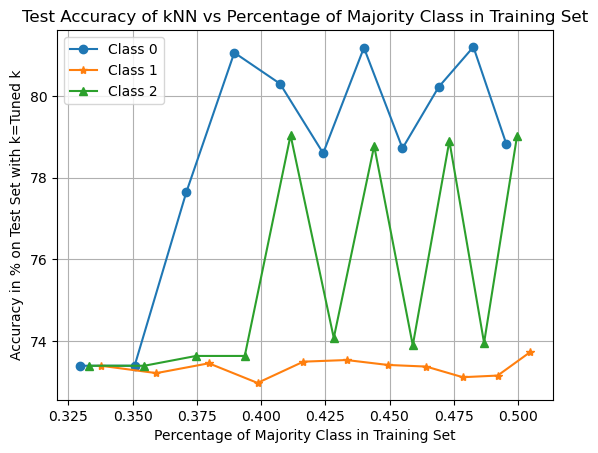
\includegraphics[width=\linewidth]{figures/f_measure_over.png}
                \caption{Representation of each class in the test set}
                \label{fig:f_over}
            \end{minipage}%
        \end{figure}

        While the F-measure is a useful metric for imbalanced datasets, it does not seem to translate well to our problem. It is possible that it is not suitable when the imbalance is artificially introduced, as in our case. The standard classification accuracy might be a more reliable metric for evaluating model performance. By removing or adding points, we are likely not reflecting the true underlying distribution, leading to skewed results using the F-measure.


\section{Conclusion}
    This project investigated the application of k-NN and various optimisation methods on the waveform dataset. Tuning the best value of $k$ results in a generalised accuracy of 84.3\%, which is quite close to the optimal Bayesian classification accuracy of 86\%, suggesting k-NN is a good algorithm for this classification problem.

    As expected, k-fold cross-validation proved to be an effective method for tuning the best value of $k$. Data reduction techniques were also successfully applied, removing outliers and redundant points, which increased the speed of k-NN predictions while maintaining a similar classification accuracy to that achieved on the original training set. Outlier removal also likely contributed to the improved accuracy of 1-NN on the reduced dataset.

    Using the triangle inequality to speed up k-NN proved to be unsuccessful. This is likely because our implementation used nested for loops, which is much less efficient than NumPy's highly optimised vectorised operations used in the brute force 1-NN. Future work could investigate an implementation of the triangle inequality using NumPy's vectorised arrays.

    Implementing sampling methods showed an imbalanced representation of the data in the test set, with one class having fewer examples than the others. Undersampling led to the expected result of the k-NN classification accuracy decreasing as the percentage of each class in the training set tends to 0. However, oversampling showed a temporary increase in accuracy when examples from the two over-represented classes were duplicated. This is likely attributed to the fact there is more examples in the training set for k-NN to match with. Using the F-measure to tune the best value of $k$ for each sampling rate did not yield the results expected, as it further reduced the test accuracy. Our conclusion is that using F-measure for artificially imbalanced datasets is not as accurate a metric as using the classification accuracy, This is possible because sampling the data alters the underlying data distribution, which deems the F-measure ineffective.

    Due to time limitations, we were unable to implement other techniques, such as PCA for dimensionality reduction. Given the correlation matrix in \ref{fig:corr_matrix}, PCA could likely retain a lot of the variance in the data with a reduced number of dimensions, potentially improving both efficiency and accuracy of k-NN.

    Future work could also include implementing more sampling methods such as SMOTE, and investigating more into the unexpected results of the triangle inequality and F-measure tuning.

    Overall, the project was a valuable insight into implementing the k-NN algorithm and applying various optimisations to it. The results show that a simple algorithm like k-NN can achieve close to the optimal Bayesian accuracy on datasets such as the waveform one. It is also important to consider and evaluate various optimisation techniques to improve the efficiency and accuracy of k-NN.




\section{Contributions}
\subsection{Patrick Barry}
\begin{itemize}
    \item Abstract, Introduction
    \item Data Exploration, Data Manipulation
    \item Task 2: Data Reduction
    \item Task 4: Sampling Methods
    \item Conclusion
\end{itemize}

\subsection{Buu Dinh Ha}
\begin{itemize}
    \item Task 1: Tuning k of k-NN by Cross Validation
    \item Task 3: Speeding up the calculation
\end{itemize}

% In the unusual situation where you want a paper to appear in the
% references without citing it in the main text, use \nocite
\nocite{langley00}

\bibliography{references}
\bibliographystyle{icml2024}

\newpage
\appendix
\onecolumn
\section{Appendices}


\begin{algorithm}[tb]
   \caption{k-folds Cross Validation}
   \label{alg:k_folds_cross_validation}
\begin{algorithmic}
   \STATE {\bfseries Input:} Dataset $\mathcal{X}_{\text{train}}$, $\mathcal{Y}_{\text{train}}$, Distance Matrix $D$, Number of Folds $k_{\text{folds}}$, Number of Neighbors $k$
   \STATE {\bfseries Output:} List of accuracies for k folds $\mathcal{A}$

   \STATE $\mathcal{F} \gets \texttt{KFoldIndices}(\mathcal{X}_{\text{train}}, k_{\text{folds}})$
   \STATE $\mathcal{A} \gets []$
   \FOR{each fold $(\mathcal{X}_{\text{train}}, \mathcal{X}_{\text{val}})$ {\bfseries in} $\mathcal{F}$}
      \STATE $D_{\text{val}} \gets \texttt{ExtractDistances}(D, \mathcal{X}_{\text{val}})$
      \STATE $\mathcal{P} \gets []$

      \FOR{each $x$ {\bfseries in} $\mathcal{X}_{\text{val}}$}
         \STATE $\mathcal{N} \gets \texttt{GetNeighbors}(D_{\text{val}}, \mathcal{X}_{\text{train}}, k)$
         \STATE $y_{\text{pred}} \gets \texttt{KnnPrediction}(\mathcal{N}, \mathcal{Y}_{\text{train}})$
         \STATE Append $y_{\text{pred}}$ to $\mathcal{P}$
      \ENDFOR

      \STATE $\mathcal{Y}_{\text{val}} \gets \texttt{GetActualLabels}(\mathcal{Y}_{\text{train}}, \mathcal{X}_{\text{val}})$
      \STATE $a \gets \texttt{AccuracyMetric}(\mathcal{Y}_{\text{val}}, \mathcal{P})$
      \STATE Append $a$ to $\mathcal{A}$
   \ENDFOR

   \STATE {\bfseries Return:} $\mathcal{A}$
\end{algorithmic}
\end{algorithm}

    \begin{algorithm}[tb]
        \caption{Remove Outliers Algorithm}
        \label{alg:remove_outliers}
        \begin{algorithmic}
           \STATE {\bfseries Input:} $X_{train}$
           \STATE {\bfseries Output:} $X_{train\_cleaned}$
           \STATE Randomly split $X_{train}$ into two subsets $S_1$ and $S_2$
           \WHILE{$S_1$ and $S_2$ not stabilised}
                \STATE Classify $S_1$ with $S_2$ using 1-NN
                \STATE Remove from $S_1$ the misclassified instances
                \STATE Classify $S_2$ with updated $S_1$ using 1-NN
                \STATE Remove from $S_2$ the misclassified instances
           \ENDWHILE
           \STATE $X_{train\_cleaned} = S_1 \cup S_2$
        \end{algorithmic}
    \end{algorithm}

    \begin{algorithm}[tb]
        \caption{Remove Redundant Points Algorithm}
        \label{alg:remove_redundancy}
        \begin{algorithmic}
           \STATE {\bfseries Input:} $X_{train}$
           \STATE {\bfseries Output:} $STORAGE$
           \STATE $STORAGE \gets \emptyset ; BIN \gets \emptyset$
           \STATE Put a random example from $X_{train}$ in $STORAGE$
           \WHILE{$STORAGE$ not stabilised}
                \FOR{all $x_i$ in $X_{train}$}
                    \STATE $y_{pred}$ = classify $x_i$ using $STORAGE$ with 1-NN
                    \IF{$y_{pred}$ is correct}
                        \STATE Add $x_i$ to $BIN$
                    \ELSE
                        \STATE Add $x_i$ to $STORAGE$
                    \ENDIF
                \ENDFOR
           \ENDWHILE
        \end{algorithmic}
    \end{algorithm}

\begin{algorithm}[tb]
   \caption{Brute Force 1-NN}
   \label{alg:brute_force_1nn}
\begin{algorithmic}
   \STATE {\bfseries Input:} Dataset  $\mathcal{X}_{\text{train}}$, $\mathcal{Y}_{\text{train}}$ , $\mathcal{X}_{\text{test}}$
   \STATE {\bfseries Output:} List of predicted labels $\mathcal{P}$ for the test set

   \STATE $\mathcal{P} \gets []$

   \FOR{$x_{\text{test}}$ {\bfseries in} $\mathcal{X}_{\text{test}}$}
       \STATE $\mathcal{D} \gets \texttt{ComputeDistances}(\mathcal{X}_{\text{train}}, x_{\text{test}})$
       \STATE $i_{\text{nearest}} \gets \texttt{FindNearestNeighbor}(\mathcal{D})$
       \STATE $y_{\text{pred}} \gets \texttt{GetLabel}(\mathcal{Y}_{\text{train}}, i_{\text{nearest}})$
       \STATE Append $y_{\text{pred}}$ to $\mathcal{P}$
   \ENDFOR

   \STATE {\bfseries Return:} $\mathcal{P}$
\end{algorithmic}
\end{algorithm}


\begin{algorithm}[tb]
   \caption{Triangle Inequality 1-NN}
   \label{alg:triangle_inequality_1nn}
\begin{algorithmic}
   \STATE {\bfseries Input:} Dataset $\mathcal{X}_{\text{train}}$, $\mathcal{Y}_{\text{train}}$, $\mathcal{X}_{\text{test}}$, distance matrix $\mathcal{D}$
   \STATE {\bfseries Output:}  List of predicted labels $\mathcal{P}$ for the test set

   \STATE $\mathcal{P} \gets []$
   \FOR{$x_{\text{test}}$ {\bfseries in} $\mathcal{X}_{\text{test}}$}
   \STATE $d_{\text{min}} \gets \infty$
       \STATE $\text{nearest\_neighbor\_label} \gets \text{None}$
       \STATE $\mathcal{C} \gets \{0, 1, \dots, n-1\}$

       \WHILE{$\mathcal{C} \neq \emptyset$}
           \STATE Select and remove the first index $i$ from $\mathcal{C}$
           \STATE $
           d_{\text{candidate}} \gets \|x_{\text{test}} - x_{\text{train}}[i]\|_2$
           \STATE
          $ \text{lower\_bound} \gets d_{\text{candidate}} - d_{\text{min}}$
          \STATE $
           \text{upper\_bound} \gets d_{\text{candidate}} + d_{\text{min}}$
           \STATE $
           d_{\text{candidate\_to\_others}} \gets \mathcal{D}[i, \mathcal{C}]$
           \STATE $
           \mathcal{C} \gets \{j \in \mathcal{C} \mid \text{lower\_bound} \leq d_{\text{candidate\_to\_others}}[j] \leq \text{upper\_bound}\}$
           \IF{$d_{\text{candidate}} < d_{\text{min}}$}
               \STATE $d_{\text{min}} \gets d_{\text{candidate}}$
               \STATE $\text{nearest\_neighbor\_label} \gets \mathcal{Y}_{\text{train}}[i]$
           \ENDIF
       \ENDWHILE
       \STATE Append $\text{nearest\_neighbor\_label}$ to $\mathcal{P}$
   \ENDFOR

   \STATE {\bfseries Return:} $\mathcal{P}$
\end{algorithmic}
\end{algorithm}

\end{document}


% This document was modified from the file originally made available by
% Pat Langley and Andrea Danyluk for ICML-2K. This version was created
% by Iain Murray in 2018, and modified by Alexandre Bouchard in
% 2019 and 2021 and by Csaba Szepesvari, Gang Niu and Sivan Sabato in 2022.
% Modified again in 2023 and 2024 by Sivan Sabato and Jonathan Scarlett.
% Previous contributors include Dan Roy, Lise Getoor and Tobias
% Scheffer, which was slightly modified from the 2010 version by
% Thorsten Joachims & Johannes Fuernkranz, slightly modified from the
% 2009 version by Kiri Wagstaff and Sam Roweis's 2008 version, which is
% slightly modified from Prasad Tadepalli's 2007 version which is a
% lightly changed version of the previous year's version by Andrew
% Moore, which was in turn edited from those of Kristian Kersting and
% Codrina Lauth. Alex Smola contributed to the algorithmic style files.
